\documentclass[10pt]{beamer}
\usetheme[progressbar=frametitle]{metropolis}
\usepackage{tikzsymbols}
\usepackage{appendixnumberbeamer}
\usepackage{booktabs}
\usepackage[scale=2]{ccicons}
\usepackage{pgfplots}
\usepackage{listings}

\usepackage{color}

\definecolor{mygreen}{rgb}{0,0.6,0}
\definecolor{mygray}{rgb}{0.5,0.5,0.5}
\definecolor{mymauve}{rgb}{0.58,0,0.82}

\lstset{ 
  backgroundcolor=\color{white},   % choose the background color; you must add \usepackage{color} or \usepackage{xcolor}; should come as last argument
  basicstyle=\footnotesize,        % the size of the fonts that are used for the code
  breakatwhitespace=false,         % sets if automatic breaks should only happen at whitespace
  breaklines=true,                 % sets automatic line breaking
  captionpos=t,                    % sets the caption-position to bottom
  commentstyle=\color{mygreen},    % comment style
  deletekeywords={...},            % if you want to delete keywords from the given language
  escapeinside={\%*}{*)},          % if you want to add LaTeX within your code
  extendedchars=true,              % lets you use non-ASCII characters; for 8-bits encodings only, does not work with UTF-8
  frame=single,	                   % adds a frame around the code
  keepspaces=true,                 % keeps spaces in text, useful for keeping indentation of code (possibly needs columns=flexible)
  keywordstyle=\color{blue},       % keyword style
  language=PHP,                 % the language of the code
  morekeywords={*,...},            % if you want to add more keywords to the set
  numbers=none,                    % where to put the line-numbers; possible values are (none, left, right)
  rulecolor=\color{black},         % if not set, the frame-color may be changed on line-breaks within not-black text (e.g. comments (green here))
  showspaces=false,                % show spaces everywhere adding particular underscores; it overrides 'showstringspaces'
  showstringspaces=false,          % underline spaces within strings only
  showtabs=false,                  % show tabs within strings adding particular underscores
  stepnumber=2,                    % the step between two line-numbers. If it's 1, each line will be numbered
  stringstyle=\color{mymauve},     % string literal style
  tabsize=2,	                   % sets default tabsize to 2 spaces
}

\usepgfplotslibrary{dateplot}
\usepackage{xspace}
\newcommand{\themename}{\textbf{\textsc{metropolis}}\xspace}
\setbeamertemplate{caption}{\raggedright\insertcaption\par}

\title{WordPress Hooks 101}
\date{Dec, 2018}
\author{Fahad Murtaza (@fahdmurtaza)}
\institute{WordCamp Biratnagar, 2018}

\begin{document}
    \maketitle

    \begin{frame}{Testing 123 ... attention please!}
        \begin{itemize}
            \item Setting the Objectives
            \item Walk away from this, feeling a little inspired and less hacky.
            \item Less spaghetti in your code. 
            \item “Eureka” moments, where suddenly your understand it and want to try it out
            \item Let’s have fun!
        \end{itemize}
    \end{frame}

    \begin{frame}{Hooks?}
        \begin{center}
            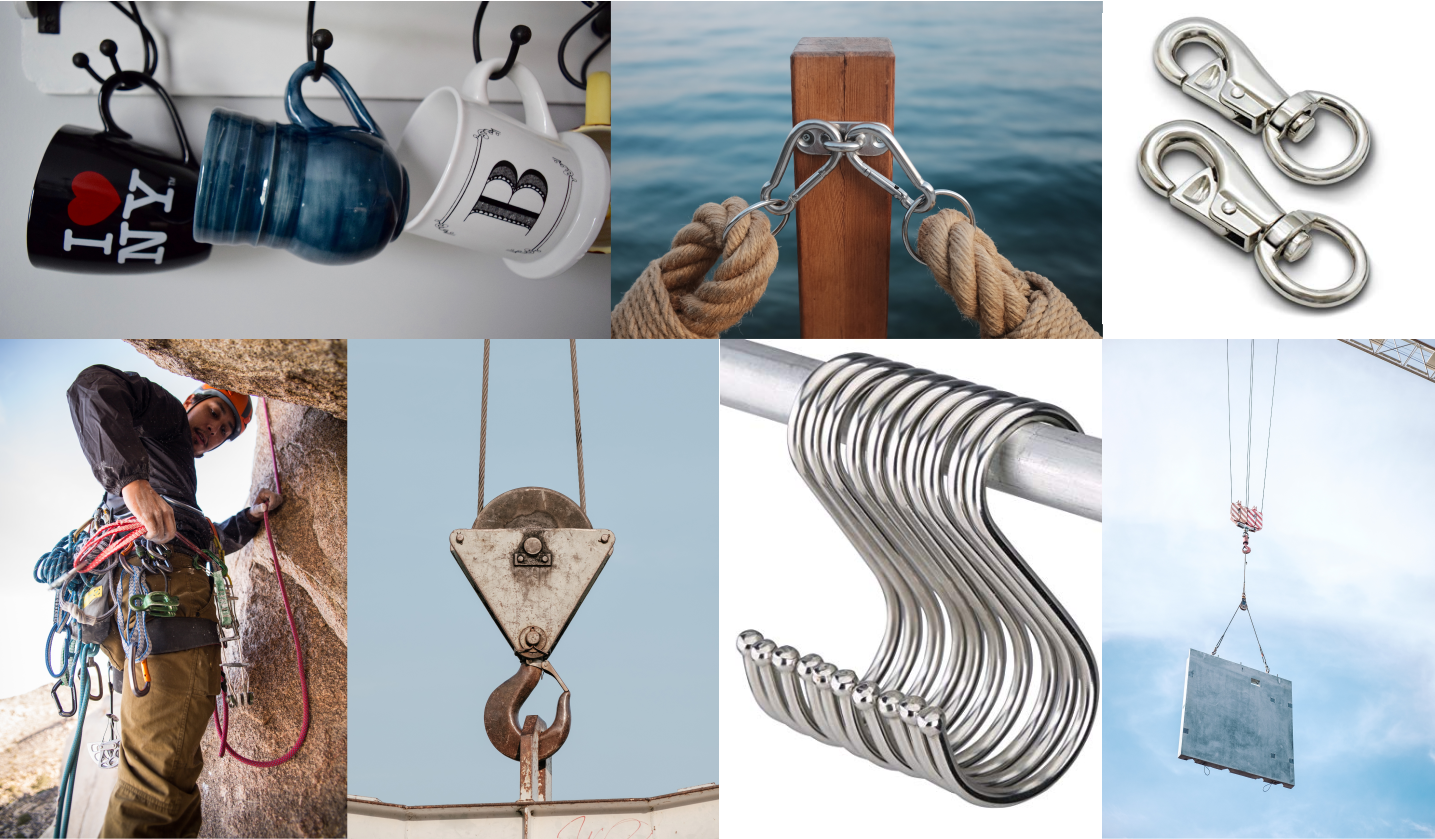
\includegraphics[width=1\textwidth]{images/hooks}
        \end{center}
    \end{frame}

    \begin{frame}{WordPress Hooks}
        \begin{large}
            Hooks are provided by WordPress to allow your plugin to 'hook into' the rest of WordPress; that is, to call functions in your plugin at specific times, and thereby set your plugin in motion.   
        \end{large}
        \begin{flushright}
            -- WordPress Codex
        \end{flushright}
    \end{frame}

    \begin{frame}{Once more!}
        \begin{large}
            ``Hooks enable us to literally hook into parts of the WordPress page lifecycle to retrieve, insert, or modify data, or they allow us to take certain actions behind the scenes..''
        \end{large}
        \begin{flushright}
            -- Tom McFlarin @ Tutsplus
        \end{flushright}
    \end{frame}

    \begin{frame}
        \begin{center}
            \begin{Huge}
                But it's more than that!
            \end{Huge}
            \vfill{}

            Can be used anywhere
            \vfill{}
            \begin{Huge}
                Themes OR Plugins
            \end{Huge}

            \vfill{}
            \metroset{block=fill}
            \begin{block}{Note}
                In case of a theme, can be used in \emph{functions.php} or a file included in \emph{functions.php} for better code organization
            \end{block}
        \end{center}
    \end{frame}

    \begin{frame}{Be Like Budh}
        \begin{columns}
            \begin{column}{0.5\textwidth}
                \begin{itemize}
                    \item[] This is Budh
                    \item[] Budh works with WordPress
                    \item[] He doesn't write spaghetti code
                    \item[] He uses WordPress Hooks
                    \item[] Be like Budh
                \end{itemize}
            \end{column}
            \begin{column}{0.5\textwidth}
                \begin{center}
                    
\includegraphics[width=1\textwidth]{images/jamal}
                \end{center}
            \end{column}
        \end{columns}
    \end{frame}

    \begin{frame}{A World without Hooks}
        \begin{columns}
            \begin{column}{0.5\textwidth}
                \begin{itemize}
                    \item Including extra PHP files for things like AJAX requests
                    \item Including files in the header / footer
                    \item Hacking into plugins to change display/functionality while you should be using a … yes … a hook
                    \item Hacking WP core files.. Seriously, who does that? 
                    \item Hacking theme files (when you should be using a child theme). With custom theme an exception to this rule.   
                \end{itemize}
            \end{column}
            \begin{column}{0.5\textwidth}
                \begin{center}
                    
\includegraphics[width=1\textwidth]{images/someasshole}
                \end{center}
            \end{column}
        \end{columns}
    \end{frame}

    \begin{frame}
        \begin{center}
            \begin{Huge}
                So... Raju
            \end{Huge}

            
\includegraphics[width=0.5\textwidth]{images/rashid}

            \begin{Huge}
                Y U No Use Hooks?
            \end{Huge}
        \end{center}
    \end{frame}

    \begin{frame}{Types of WordPress Hooks}
        \begin{columns}
            \begin{column}{0.5\textwidth}
                \begin{center}
                    \begin{Huge}
                        Filters
                    \end{Huge}
                \end{center}
            \end{column}
            \begin{column}{0.5\textwidth}
                \begin{center}
                    \begin{Huge}
                        Actions
                    \end{Huge}
                \end{center}
            \end{column}
        \end{columns}
    \end{frame}

    \begin{frame}{Filters and Actions}
        \begin{columns}
            \begin{column}{0.5\textwidth}
                \begin{center}
                    \begin{Huge}
                        Filters
                    \end{Huge}
                \end{center}                    
                \begin{figure}
                \lstinputlisting[title=Applying changing to content]{filters.php}
                \end{figure}
            \end{column}
            \begin{column}{0.5\textwidth}
                \begin{center}
                    \begin{Huge}
                        Actions
                    \end{Huge}
                \end{center}                    
                \begin{figure}
                \lstinputlisting[title=Hook your functions into an action]{actions.php}
                \end{figure}
            \end{column}
        \end{columns}
    \end{frame}

    \begin{frame}
        \begin{center}
            \begin{Huge}
                But they sound so similar?
            \end{Huge}

            \vfill{}
            
\includegraphics[width=0.8\textwidth]{images/similar}
        \end{center}
    \end{frame}

    \begin{frame}{Yes they are ... except!}
        Filters and actions are almost the same thing in syntax and capabilities but:
        \begin{itemize}
            \item The difference is how you use them!
            \item Both are powerful but remember:
        \end{itemize}
        \metroset{block=fill}
        \begin{alertblock}{Caution}
            ``With great power comes great responsibility'' -- Not Uncle Ben
        \end{alertblock}
    \end{frame}

    \begin{frame}
        \begin{columns}
            \begin{column}{0.5\textwidth}
                \begin{center}
                    \begin{Huge}
                        Filters
                    \end{Huge}
                \end{center}
                \begin{itemize}
                    \item Change existing WordPress content, blog posts, text, media files etc. Like cropping text or modifying a word.
                    \item Change database content on the fly or display it differently
                    \item Clean up poorly formatted code b ‘filtering out’ certain tags
                \end{itemize}
            \end{column}
            \begin{column}{0.5\textwidth}
                \begin{center}
                    \begin{Huge}
                        Actions
                    \end{Huge}
                \end{center}
                \begin{itemize}
                    \item Tying into existing WordPress processes, like creating a new user, saving a post, updating permalinks, sending emails, saving a comment, etc. 
                    \item Adding an action to your plugin / theme to allow other developers to manipulate it without hacking 
                \end{itemize}
            \end{column}
        \end{columns}
    \end{frame}

    \begin{frame}
        \begin{center}
            \begin{Huge}
                Makes a little more sense now!
            \end{Huge}

            \vfill{}
            
\includegraphics[width=1\textwidth]{images/sense}
        \end{center}
    \end{frame}

    \begin{frame}{Code Demos}
        \begin{itemize}
            \item Sending all email notifications from gravity forms when a form is submitted
            \item Send an email on a post update
            \item Send an email on a post create / publish
            \item Reset the permalinks on a new custom post type registration 
            \item Filtering the bad words from content
            \item Resizing the image
        \end{itemize}
    \end{frame}

    \begin{frame}
        \lstinputlisting{code1.php}
    \end{frame}

    \begin{frame}
        \lstinputlisting{code2.php}
    \end{frame}

    \begin{frame}
        \lstinputlisting{code3.php}
    \end{frame}
    
    \begin{frame}
        \lstinputlisting{code5.php}
    \end{frame}

    \begin{frame}
        \lstinputlisting{code6.php}
    \end{frame}
    
    \begin{frame}[standout]
        \begin{Huge}
            Questions?
        \end{Huge}

        \vfill{}
        ``For everything you know, there are many more people out there that don't know.''
        
        \vfill{}
        \begin{large}
            Don't be shy!
        \end{large}

        \vfill{}

        \begin{center}
            info@fahdmurtaza.com 

            (@fahdmurtaza)

            https://goo.gl/xb5deC
        \end{center}
    \end{frame}
\end{document}